\documentclass[border=4pt,12pt]{standalone}
% House style for redrawn exam diagrams (diagram-v4: 0.4pt lines, filled -latex arrows, fine dashes; stipple and hatching drawn as real dots/lines (no PDF/SVG patterns, so they render in every browser and at any scale); transparent background). Every figure \input's this.
\usepackage{amsmath,amssymb}
\usepackage{txfonts}
\usepackage{pdfrender,xcolor}
% \halo{text}: label on shading. The shading stops just around each letter's outline (a thin knock-out that follows the
% glyphs, like the papers' typesetting), never a box. Owner: "I don't want a box around the text".
\newcommand{\halo}[1]{\leavevmode\rlap{\pdfrender{TextRenderingMode=2,LineWidth=2.2pt,LineJoinStyle=1,StrokeColor=white,FillColor=white}#1}#1}
\usepackage{tikz,pgfplots}
\pgfplotsset{compat=1.18}
\usetikzlibrary{arrows.meta,calc,angles,quotes,patterns,patterns.meta,intersections,positioning,decorations.markings,shapes.geometric}
% Stipple and hatching are drawn as actual dots / lines clipped to the region (path picture), NOT as pattern fills:
% SVG <pattern> fills vanish or blur when browsers scale the image, so the owner could not see the shading.
% Each dot is a 0.72pt square (keeps SVGs small; reads as a dot at print size). Dots sit on one global staggered grid, so neighbouring regions line up.
\makeatletter
\newdimen\ex@x \newdimen\ex@y \newdimen\ex@xa \newdimen\ex@ya \newdimen\ex@xb \newdimen\ex@yb \newcount\ex@row
\def\exam@stipplecolor{black!75}\def\exam@dotr{0.42pt}\def\exam@dotgap{2.5}
\def\ex@rowdots{\ifdim\ex@x<\ex@xb \pgfpathrectangle{\pgfqpoint{\dimexpr\ex@x-0.36pt\relax}{\dimexpr\ex@y-0.36pt\relax}}{\pgfqpoint{0.72pt}{0.72pt}}\advance\ex@x by \exam@dotgap pt\relax\expandafter\ex@rowdots\fi}
\def\exam@stipple{%
  \pgftransformreset% dots are sized in real points even inside scaled pictures
  \pgfpointanchor{path picture bounding box}{south west}\ex@xa=\pgf@x \ex@ya=\pgf@y
  \pgfpointanchor{path picture bounding box}{north east}\ex@xb=\pgf@x \ex@yb=\pgf@y
  \pgfsetfillcolor{\exam@stipplecolor}\pgfmathsetmacro\ex@h{\exam@dotgap/2}%
  \pgfmathtruncatemacro\ex@r{floor(\ex@ya/\ex@h)-1}\ex@row=\ex@r\relax
  \ex@y=\ex@r\dimexpr\ex@h pt\relax
  \loop\ifdim\ex@y<\ex@yb
    \pgfmathtruncatemacro\ex@c{floor(\ex@xa/\exam@dotgap)-1}\ex@x=\ex@c\dimexpr\exam@dotgap pt\relax
    \ifodd\ex@row \advance\ex@x by \ex@h pt\fi
    \ex@rowdots
    \advance\ex@y by \ex@h pt \advance\ex@row by 1
    \ifnum\numexpr\ex@row-(\ex@row/4)*4\relax=0 \pgfusepath{fill}\fi% flush every 4 rows: bounded TeX memory, few clip copies in the SVG
  \repeat\pgfusepath{fill}}
\newdimen\ex@d
\def\exam@hatch#1{% #1 = 1 for /, -1 for \ ; lines 45 degrees, 3pt apart
  \pgftransformreset
  \pgfpointanchor{path picture bounding box}{south west}\ex@xa=\pgf@x \ex@ya=\pgf@y
  \pgfpointanchor{path picture bounding box}{north east}\ex@xb=\pgf@x \ex@yb=\pgf@y
  \ex@d=\dimexpr\ex@yb-\ex@ya\relax \ex@x=\dimexpr\ex@xa-\ex@d\relax
  \loop\ifdim\ex@x<\ex@xb
    \ifnum#1>0 \pgfpathmoveto{\pgfqpoint{\ex@x}{\ex@ya}}\pgfpathlineto{\pgfqpoint{\dimexpr\ex@x+\ex@d\relax}{\ex@yb}}%
    \else \pgfpathmoveto{\pgfqpoint{\ex@x}{\ex@yb}}\pgfpathlineto{\pgfqpoint{\dimexpr\ex@x+\ex@d\relax}{\ex@ya}}\fi
    \advance\ex@x by 4.24pt
  \repeat
  \pgfsetlinewidth{0.4pt}\pgfsetstrokecolor{black}\pgfusepath{stroke}}
\def\examstipple{\exam@stipple}\def\examhatch{\exam@hatch}\def\examsetstipplecolor#1{\def\exam@stipplecolor{#1}}\def\examsetdotgap#1{\def\exam@dotgap{#1}}
\makeatother
% (legacy pattern kept for old files)
% staggered stipple like the NESA papers' dotted shading
\pgfdeclarepatternformonly{exam stipple}{\pgfpointorigin}{\pgfqpoint{2.2pt}{2.2pt}}{\pgfqpoint{2.2pt}{2.2pt}}{%
  \pgfpathcircle{\pgfqpoint{0.55pt}{0.55pt}}{0.42pt}\pgfpathcircle{\pgfqpoint{1.65pt}{1.65pt}}{0.42pt}\pgfusepath{fill}}
\tikzset{
  every picture/.style={line width=0.6pt, >={Latex[length=2mm,width=1.3mm]}},
  curve/.style={line width=0.6pt},
  open arrow/.style={-{Latex[length=2mm,width=1.3mm]}},  % owner: filled -latex heads everywhere, no open chevrons
  aux/.style={dash pattern=on 2pt off 1.5pt, line width=0.6pt},
  shade/.code={\def\exA{#1}\def\exB{none}\ifx\exA\exB\else\pgfkeysalso{fill=black!18}\fi},
  shade/.default=on,
  shade dots/.style={fill=none, path picture={\examstipple}},
  stipple color/.code={\examsetstipplecolor{#1}},
  stipple gap/.code={\examsetdotgap{#1}},
  shade dense dots/.style={fill=none, stipple gap=1.6, path picture={\examstipple}},
  shade hatch/.style={fill=none, path picture={\examhatch{1}}},
  shade hatch reverse/.style={fill=none, path picture={\examhatch{-1}}},
  shade solid/.style={fill=black},
  pt/.style={circle, fill, inner sep=1.1pt},
  open pt/.style={circle, draw, fill=white, inner sep=1.1pt},
}
\pgfplotsset{
  exam axes/.style={axis lines=middle, axis line style={->}, xlabel={$x$}, ylabel={$y$},
    xlabel style={anchor=west}, ylabel style={anchor=south}, tick label style={font=\small},
    every axis plot/.append style={line width=0.6pt, black}, samples=200, clip=false,
    enlargelimits=false, axis on top},
}

\begin{document}
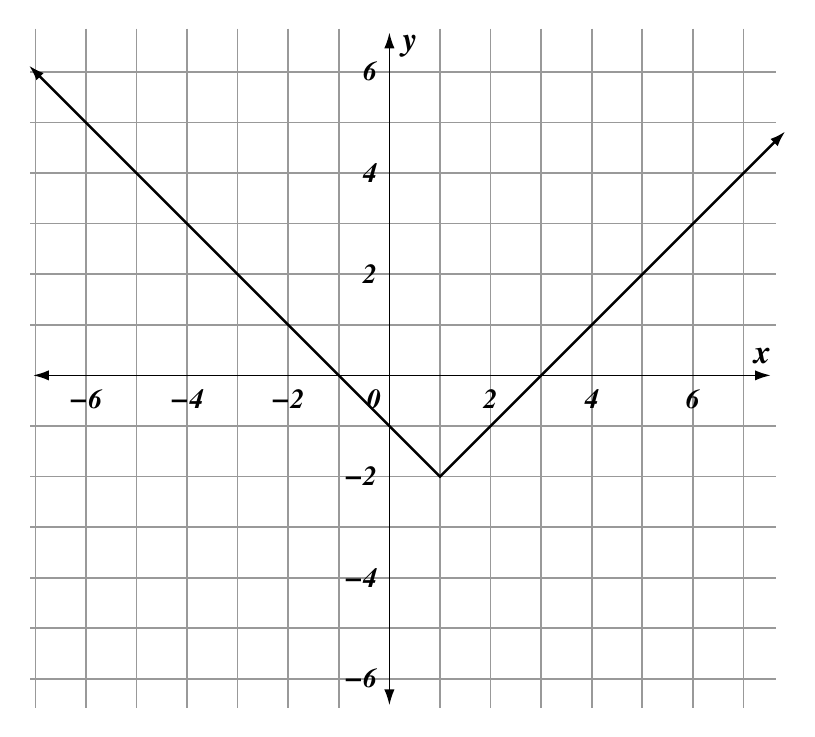
\begin{tikzpicture}[x=0.0127cm,y=-0.0127cm,font=\fontsize{10}{12}\selectfont\bfseries\itshape]
\newcommand{\lab}[1]{\ifnum#1<0 $\boldsymbol{-}$\the\numexpr-#1\relax\else#1\fi}
\begin{scope}[black!40]
\draw (21.3,21.0) -- (21.3,701.0);
\draw (71.9,21.0) -- (71.9,701.0);
\draw (16.0,671.6) -- (762.0,671.6);
\draw (122.5,21.0) -- (122.5,701.0);
\draw (16.0,621.0) -- (762.0,621.0);
\draw (173.1,21.0) -- (173.1,701.0);
\draw (16.0,570.4) -- (762.0,570.4);
\draw (223.7,21.0) -- (223.7,701.0);
\draw (16.0,519.8) -- (762.0,519.8);
\draw (274.3,21.0) -- (274.3,701.0);
\draw (16.0,469.2) -- (762.0,469.2);
\draw (324.9,21.0) -- (324.9,701.0);
\draw (16.0,418.6) -- (762.0,418.6);
\draw (426.1,21.0) -- (426.1,701.0);
\draw (16.0,317.4) -- (762.0,317.4);
\draw (476.7,21.0) -- (476.7,701.0);
\draw (16.0,266.8) -- (762.0,266.8);
\draw (527.3,21.0) -- (527.3,701.0);
\draw (16.0,216.2) -- (762.0,216.2);
\draw (577.9,21.0) -- (577.9,701.0);
\draw (16.0,165.6) -- (762.0,165.6);
\draw (628.5,21.0) -- (628.5,701.0);
\draw (16.0,115.0) -- (762.0,115.0);
\draw (679.1,21.0) -- (679.1,701.0);
\draw (16.0,64.4) -- (762.0,64.4);
\draw (729.7,21.0) -- (729.7,701.0);
\end{scope}
\draw[<->] (19.0,368.0) -- (757.0,368.0);
\draw[<->] (375.5,698.0) -- (375.5,25.0);
\def\ox{375.50}\def\oy{368.00}\def\u{50.600}
\node[anchor=north,inner sep=2pt] at (71.9,376.0) {\lab{-6}};
\node[anchor=east,inner sep=2pt] at (369.5,671.6) {\lab{-6}};
\node[anchor=north,inner sep=2pt] at (173.1,376.0) {\lab{-4}};
\node[anchor=east,inner sep=2pt] at (369.5,570.4) {\lab{-4}};
\node[anchor=north,inner sep=2pt] at (274.3,376.0) {\lab{-2}};
\node[anchor=east,inner sep=2pt] at (369.5,469.2) {\lab{-2}};
\node[anchor=north,inner sep=2pt] at (476.7,376.0) {\lab{2}};
\node[anchor=east,inner sep=2pt] at (369.5,266.8) {\lab{2}};
\node[anchor=north,inner sep=2pt] at (577.9,376.0) {\lab{4}};
\node[anchor=east,inner sep=2pt] at (369.5,165.6) {\lab{4}};
\node[anchor=north,inner sep=2pt] at (679.1,376.0) {\lab{6}};
\node[anchor=east,inner sep=2pt] at (369.5,64.4) {\lab{6}};
\node[anchor=north east,inner sep=2pt] at (373.5,376.0) {0};
\node[anchor=south west,inner sep=1pt] at (735.0,360.0) {\fontsize{12}{14}\selectfont$\boldsymbol{x}$};
\node[anchor=west,inner sep=1pt] at (383.5,39.0) {\fontsize{12}{14}\selectfont$\boldsymbol{y}$};
\begin{scope}[shift={(\ox,\oy)},x=0.643cm,y=0.643cm]
\draw[<->,line width=0.9pt] (-7.12,6.12) -- (1,-2) -- (7.82,4.82);
\end{scope}

\end{tikzpicture}
\end{document}
